
\bibliographystyle{unsrtnat}

\chapter{Literature Review}
\label{chap:LiteratureReview}

In this chapter, an analysis of previous work completed in the field of swarm robotics and biologically inspired engineering is provided, as well as an outline of the theoretical concepts concerning the techniques applied during this project.

\section{Biologically Inspired Computation and Engineering}

Nature has provided examples of outwardly complex biological systems which are often efficient, fluid and resilient to partial breakdowns. Colonies of ants are able to forage for food and build large, complex structures. Fireflies are able to synchronize their flashing with one another. Flocks of birds and schools of fish exhibit fluid and efficient group movement. In the majority of cases, nature has achieved these despite utilizing very little to no communication between individual creatures and in the absence of a higher level director or supervisor. The animals react only to environmental stimuli, either the strength or type of pheromones detected in the environment in the case of ants (termed \textsl{stigmergy}) or the positions of other individuals in the case of fish and birds. For example, it has been shown that over time, the velocity of a flock of birds converges to a state where each individual has equal velocity. \cite{cucker-smale}

This is defined as \textsl{emergent behaviour}, the rise of previously unpredicted and complex behaviour through the interaction of simple rules.

Researchers have attempted to replicate this in an artificial system via various means. For example, Bojinov et. al (2000) demonstrated how simple, local sensory rules can produce complex and useful structures in metamorphic robots. \cite{Bojinov2000} Metamorphic, or modular, robots are a relatively new concept which can be described as "a robot that is composed of modules that are all identical". \cite{Yim} In their paper, Bojinov et. al explored the use of purely \textit{local} rules and interactions to develop control algorithms which enabled a Proteo robot to accomplish some otherwise difficult and complex tasks. Such tasks include forming three dimensional structures, locomotion and dynamic adaptation.

Previous work on this front has utilised an exact, a-priori definition of the configuration of the robot, calculated via algorithms that use heuristics. \cite{metricsrob} These algorithms all require knowledge of the problem, the environment and the desired shape before hand, which in a real world setting is not always feasible.  What makes the work of Bojinov et. al interesting is that their algorithm does not aim to produce a pre-defined shape, rather it aims to produce a shape with the desired \textsl{properties} needed to solve the problem at hand. In this way, the algorithm produced is robust to unknowns, noise or changes in the environment, in a similar manner to how animals can adapt to changes in their environment. 

Taking advantage of the solutions to problems that nature has already solved and applying these in order to tackle similar problems in industry can be of great benefit to a engineer. While this effect can be seen in a wide range of fields, perhaps the biggest effect of biologically inspired engineering can be seen in the field of medical rehabilitation or human augmentation. 

A particular area of interest to researchers and industry alike is the development of devices that can assist the lower body in performing work. Harvard University's Wyss Institute have developed several iterations of an assistive wearable robot - an exoskeleton - that can aid in load carrying, performance enhancing and even some medical applications. \cite{soft-exo} Where their approach differs is the use of textiles in place of more rigid materials such as aluminium or carbon. In this way, they avoid the problem of having imperfectly aligned rigid links interfering with the movement of biological joints and adding inertia to the legs. Inertia can significantly increased the metabolic cost of moving the legs, an 8\% increase per kilogram at the legs versus a 1-2\% increase per kilogram at the waist. \cite{soft-exo} The Wyss Institute's earlier design relied on penumatic tubes which support the movement of the joints in the legs. Compared to more rigid designs, this provides a lightweight and low profile system with little effects on a user's kinematics. However, this comes at the cost of only being able to supply tensile forces and a significant reduction in maximum torques (1-10 times biological normal for rigid systems vs 0.1-1 times biological normal for soft systems). The most recent design operates on a similar principle, however it eschews pneumatics in favour of Bowden cables actuated by motors. This further reduces bulk, as compressed air is no longer needed and the cables are of a lower profile than pneumatic muscles.

As shown, applying biologically inspired techniques has to date been largely successful, with promising results from both academia and industry. 

\section{Artificial Intelligence and Artificial Life}
One of the most expansive fields in computer science, artificial intelligence (AI) has decades of history and continues to be a hotly researched topic for academics and industry professionals alike. The field is defined as the study of intelligent agents, however where it differs from other attempts to understand intelligent agents (such as psychology or philosophy) is that AI seeks to construct them too. \cite{russell-norvig}

It is a common misconception of artificial intelligence that it is the search and development of purely "human-like" behaviour and thinking. Indeed, countless stories and movies portray this as fact. However, while the development and research into so called "strong AI" is prevalent and cutting edge, there are many domains within AI and a huge array of techniques that can be applied. 

A notable technique in AI research is the artificial neural network (ANN). This strives to model the way a biological brain performs a given task, such as vision, hearing and actuation. An artificial neural network is composed of multiple simple computation nodes (neurons), each passing  an input (or a combination of inputs) through an activation function which determine the value of the output. It is through the interconnected nature of these neurons that give rise to the computational power of a neural network. \cite{haykin2009neural} 

ANNs have been used extensively since their conception, with applications ranging from function approximation to operating as a robot controller.

One of the major reasons for continued AI development is to act as a decision making tool that is many times faster than a human could ever achieve. With a rise in greater computational power coupled with a decrease in hardware size and cost, AI has become an increasingly ubiquitous tool that many companies and researches are utilising. For example, Amazon's development of transactional AI - which analyses the shopping habits of customers and uses this to make predictions on future purchases - has allowed the company to generate a substantial amount of profit. Another use of AI is in the operation of autonomous vehicles, which greatly benefits from a computer's fast reaction time and inability to become tired, bored or lose focus. Google, Tesla and a host of other technology and car manufacturers are investing significant capital into realising a safe autonomous system. For example, Tesla's Model S has all of the necessary hardware (such as sensors and actuators) built in for it to function as a fully autonomous vehicle, it just requires the correct software implementation. \cite{tesla}

Differing from artificial intelligence, is the field of artificial \textit{life} (AL, or ALife), which concerns itself with the study of systems relating to biological life and it's processes through computer ``simulation, robotics, or biochemistry''. \cite{artlife} First coined in 1986 by theoretical biologist and one of the founders of the discipline Christopher Langton \cite{langton}, the field differs from AI. Where AI seeks to study intelligence, AL seeks to study the fundamental processes of living systems. 

There are three approaches to AL research: ``soft'' (software based approaches such as simulations), ``hard'' (hardware based approaches such as robotics) and ``wet'' (the application of biochemistry). Each approach has it's own pros and cons, though many researchers are turning to simulation based studies to reduce time and the possibility of hardware issues.

\textit{Vehicles: Experiments in Synthetic Psychology} by Valentino Braitenberg, a book acclaimed among roboticists and social scientists alike, describes a thought experiment in which simple vehicles (now known as Braitenberg vehicles) can ``exhibit behaviors akin to aggression, love, foresight, and optimism''. \cite{braitenberg1986vehicles} In its most simple configuration, a vehicle has primitive sensors (often light sensors) connected directly to the wheels. The vehicle then does nothing more than move its wheels for a given sensor input. Therefore, depending on the wiring of the sensors to the actuators, the vehicles exhibit different behaviours, such as light following or light avoidance all with varying speeds and directions. 

As computer simulation technology improved, Braitenberg's thought experiment was validated as true. In an environment with many sources of stimulus, the vehicles can produce complex behaviour, which despite its simple internals can appear as if under intelligent control.

\section{Swarm Intelligence and Behaviour}

In 1989, Gerardo Beni and Jin Wang coined the termed \textit{swarm intelligence} in their paper \textit{Swarm Intelligence in Cellular Robotic Systems} and Beni has authored several books on the subject of swarm robotics.

Swarm intelligence is defined as the collective behavior of self-organizing and decentralized natural or artificial systems, arising through the interactions between simple agents. \cite{Beni1989} Beni states that the term was applied due to the similarities between his simulated cellular robots and social insects, notably: ``decentralised control, lack of synchronicity, simple and (quasi) identical members''. Another important aspect of swarm systems is the concept of self-organization, which was encapsulated by Bonabeau et al (1999): ``self-organisation is a set of dynamical mechanisms whereby structures appear at the global level of a system from interactions among its lower-level components''. \cite{bonabeau} What this means is that the rules which govern the interactions within a self-organising system are executed using purely local information and without knowledge of any global/system wide stimulus. This means that any pattern that arises at a global level is an emergent property of the system, as opposed to something dictated by a higher level supervisor. 

For example, a single ant operating by itself does not exhibit behaviour more complex than simply wandering around the immediate environment, lost. However, an \textit{ant colony}, operating as one system are capable of complex feats that no individual ant is capable of performing, despite the lack of an overall co-ordinator. \cite{ants} A colony can expand or contract its territory, which will effect the patrol routes of guard ants, which in turn effect the routes of the foragers and so on. In this manner, an ant colony is said to be largely self-organising and the patterns emergent.

For this reason, ants are extremely interesting to researchers. Ants communicate via a process called \textit{stigmergy}, in which they detect the pheromones left behind by other ants and based on this, decide what they should next do. This process can be replicated within an artificial system and has given rise to optimisation techniques based on environmental stimuli, such as Ant Colony Optimisation.

As can be seen, perhaps the most defining characteristic of a swarm system is emergent behavior. 

One of the most prominent examples of emergent behavior in the field is the development of the artificial life program \textit{Boids}, developed by Craig Reynolds in 1986. This provides a realistic simulation of the flocking behavior of birds through the interaction of agents present in the system.

At its most basic level Reynolds, in his paper \textit{Flocks, herds and schools: A distributed behavioral model}, defined the rules followed by all individual agents as \cite{Reynolds:1987:FHS:37402.37406}:

\begin{enumerate}
	\item \textit{Separation}: move to avoid crowding local flockmates
	\item \textit{Alignment}: steer towards the average heading of local flockmates
	\item \textit{Cohesion}: steer to move toward the average position of local flockmates
\end{enumerate}

This concept of locality means that agents do not react to the system as a whole, but only to agents within a certain radius - a neighborhood. This could model a creature’s limited perception of its surroundings or its section of the environment in which to draw stimuli from.

Originally developed as a means to provide natural movements of various animals in computer graphics,
the \textit{Boids} model has now seen extensive use in a multitude of applications from games development to military vehicles, task optimization and swarm robotics. It is this set of rules that the robot controller of this project will be based upon.

\begin{figure}[h]
	\centering
	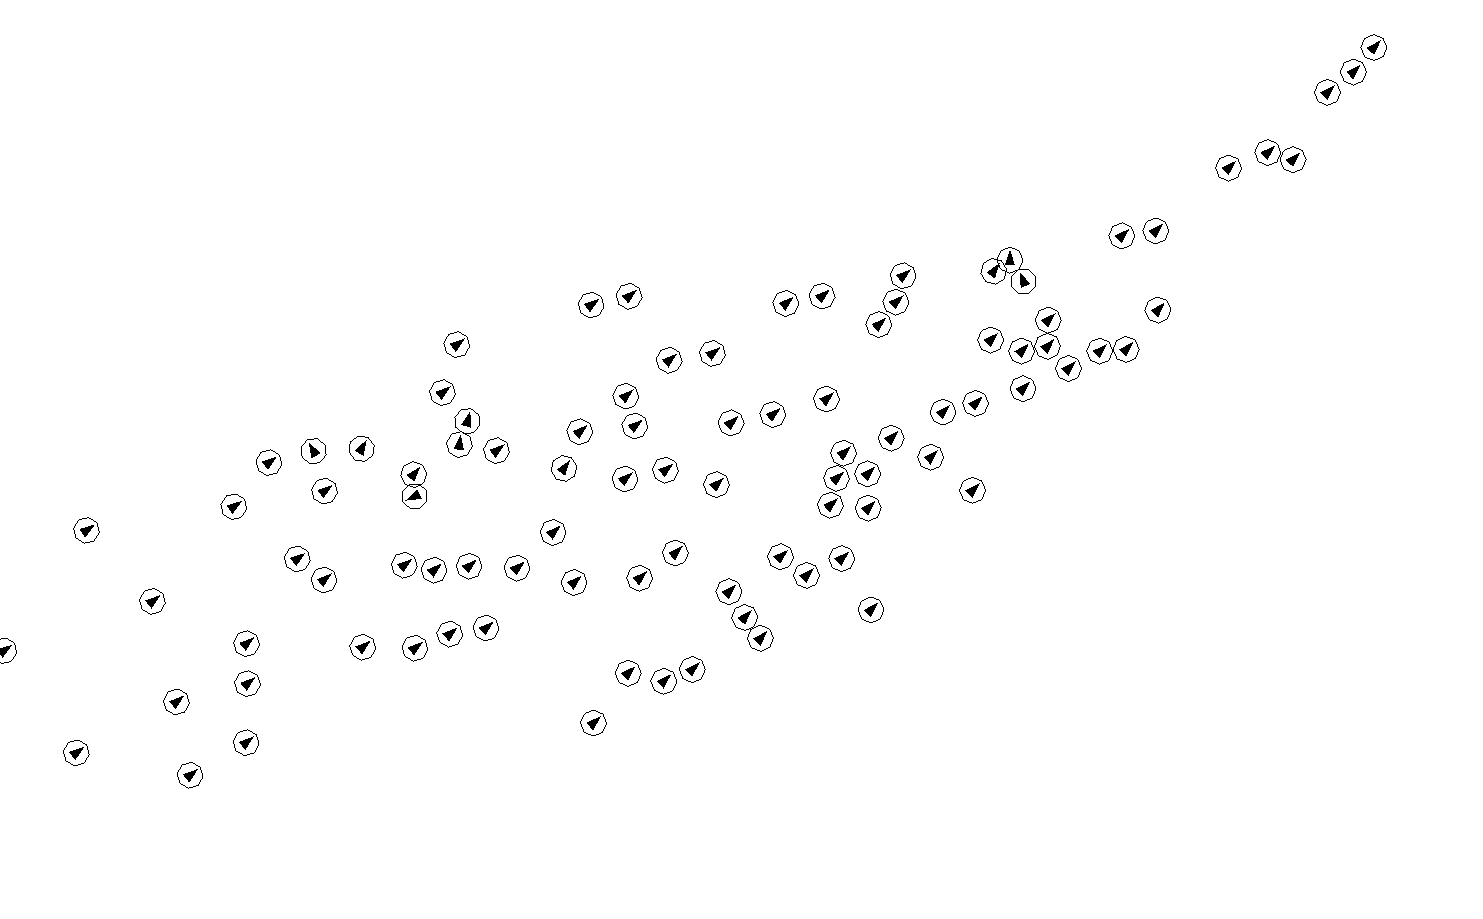
\includegraphics[width=1\textwidth]{boids}
	\caption{\label{fig:boid}A demonstration of boids}
\end{figure}